%%%%%%%%%%%%%%%%%%%%%%%%%%%%%%%%%%%%%%%%%%%%%%%%%%%%%%%%%%%%%%%%%%%%%%%%%%%%%%%%%%%%%%%%%%%%%%%%%%%%%%%%%%%%%%%%%%%%%%%%%%%%%%%%%%%%%%%%%%%%%%%%%%%%%%%%%%%
% This is just an example/guide for you to refer to when producing your supplementary material for your Frontiers article.                                 %
%%%%%%%%%%%%%%%%%%%%%%%%%%%%%%%%%%%%%%%%%%%%%%%%%%%%%%%%%%%%%%%%%%%%%%%%%%%%%%%%%%%%%%%%%%%%%%%%%%%%%%%%%%%%%%%%%%%%%%%%%%%%%%%%%%%%%%%%%%%%%%%%%%%%%%%%%%%

%%% Version 2.5 Generated 2018/06/15 %%%
%%% You will need to have the following packages installed: datetime, fmtcount, etoolbox, fcprefix, which are normally inlcuded in WinEdt. %%%
%%% In http://www.ctan.org/ you can find the packages and how to install them, if necessary. %%%
%%%  NB logo1.jpg is required in the path in order to correctly compile front page header %%%

%\documentclass[utf8]{frontiers_suppmat} % for all articles
%\usepackage{url,hyperref,lineno,microtype}
%\usepackage[onehalfspacing]{setspace}



% Leave a blank line between paragraphs instead of using \\

%\begin{document}
%\onecolumn
%\firstpage{1}

%\title {{\helveticaitalic{Supplementary Material}}}


%\maketitle

%\section{Supplementary Tables and Figures}

\section{Figures}

\begin{figure}[htbp]
\begin{center}
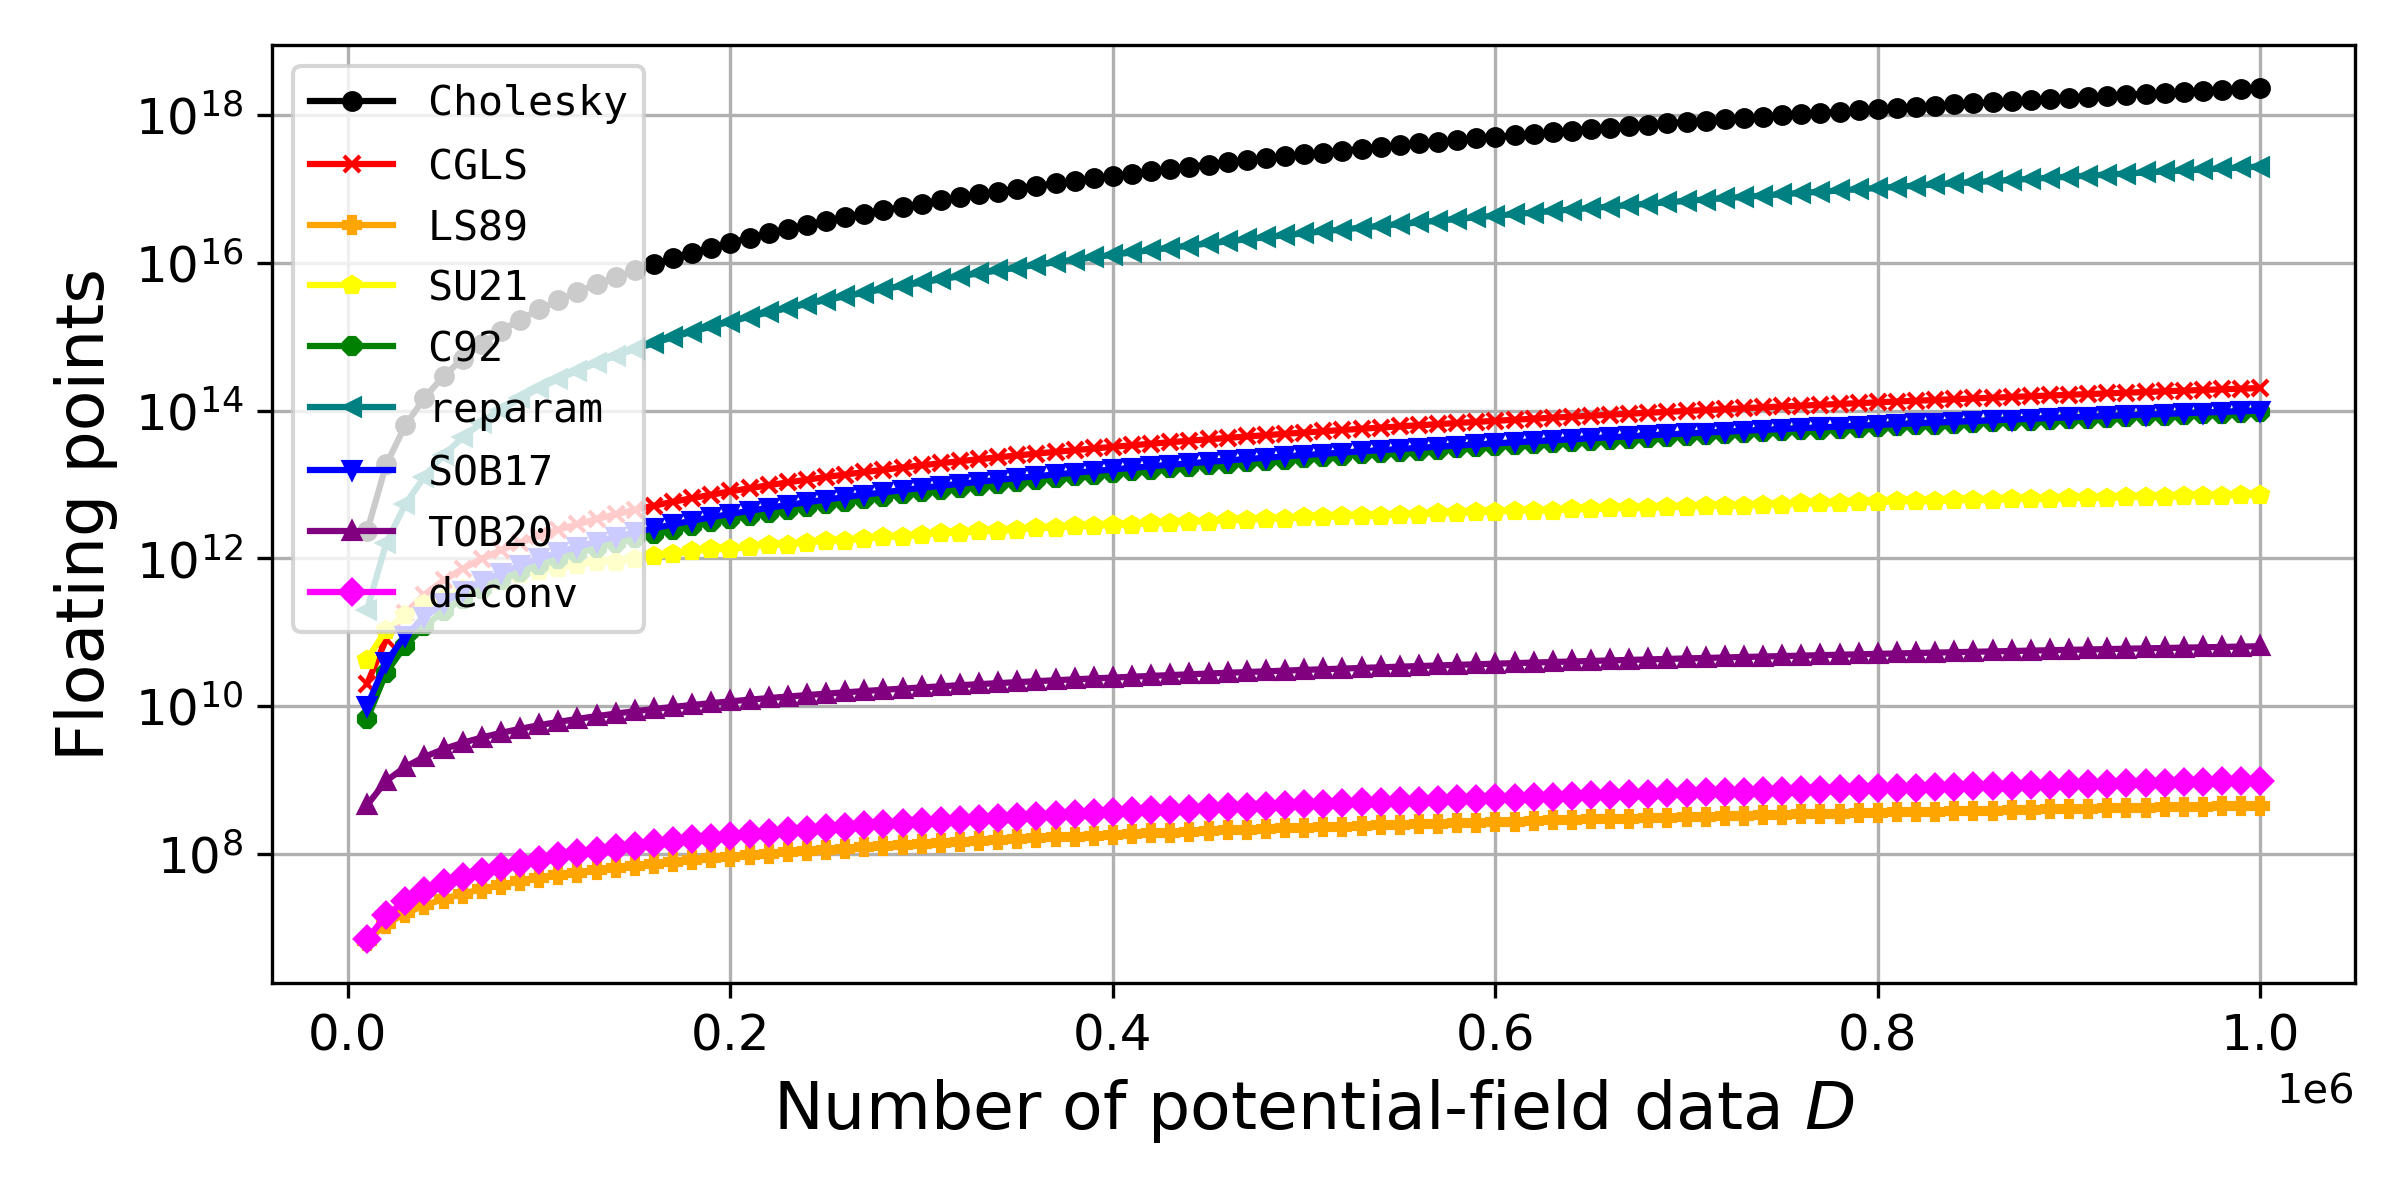
\includegraphics[width=9cm]{Fig/flops}% This is a *.eps file
\end{center}
\caption{
	Total number of flops for different equivalent-layer methods
	(equations \ref{flops:cholesky}, \ref{flops:cgls}, \ref{flops:LS89}, \ref{flops:SU21}, 
	\ref{flops:C92}, \ref{flops:reparameterization-cgls}, \ref{flops:SOB17}, \ref{flops:TOB20},
	and \ref{flops:direct-deconv}). 
	The number of potential-field data $D$ varies from $10,000$ to $1,000,000$.
	}
\label{fig:flops}
\end{figure}

%\begin{figure}[htbp]
%	\begin{center}
%		\includegraphics[width=9cm]{Fig/flops_mag}% This is a *.eps file
%	\end{center}
%	\caption{Number of \textit{flops} for many of the methods described in this work to estimate the equivalent sources using magnetic data. The range of observations varies from $10,000$ to $1,000,000$.}
%	\label{fig:2}
%\end{figure}

\begin{figure}[htbp]
	\begin{center}
			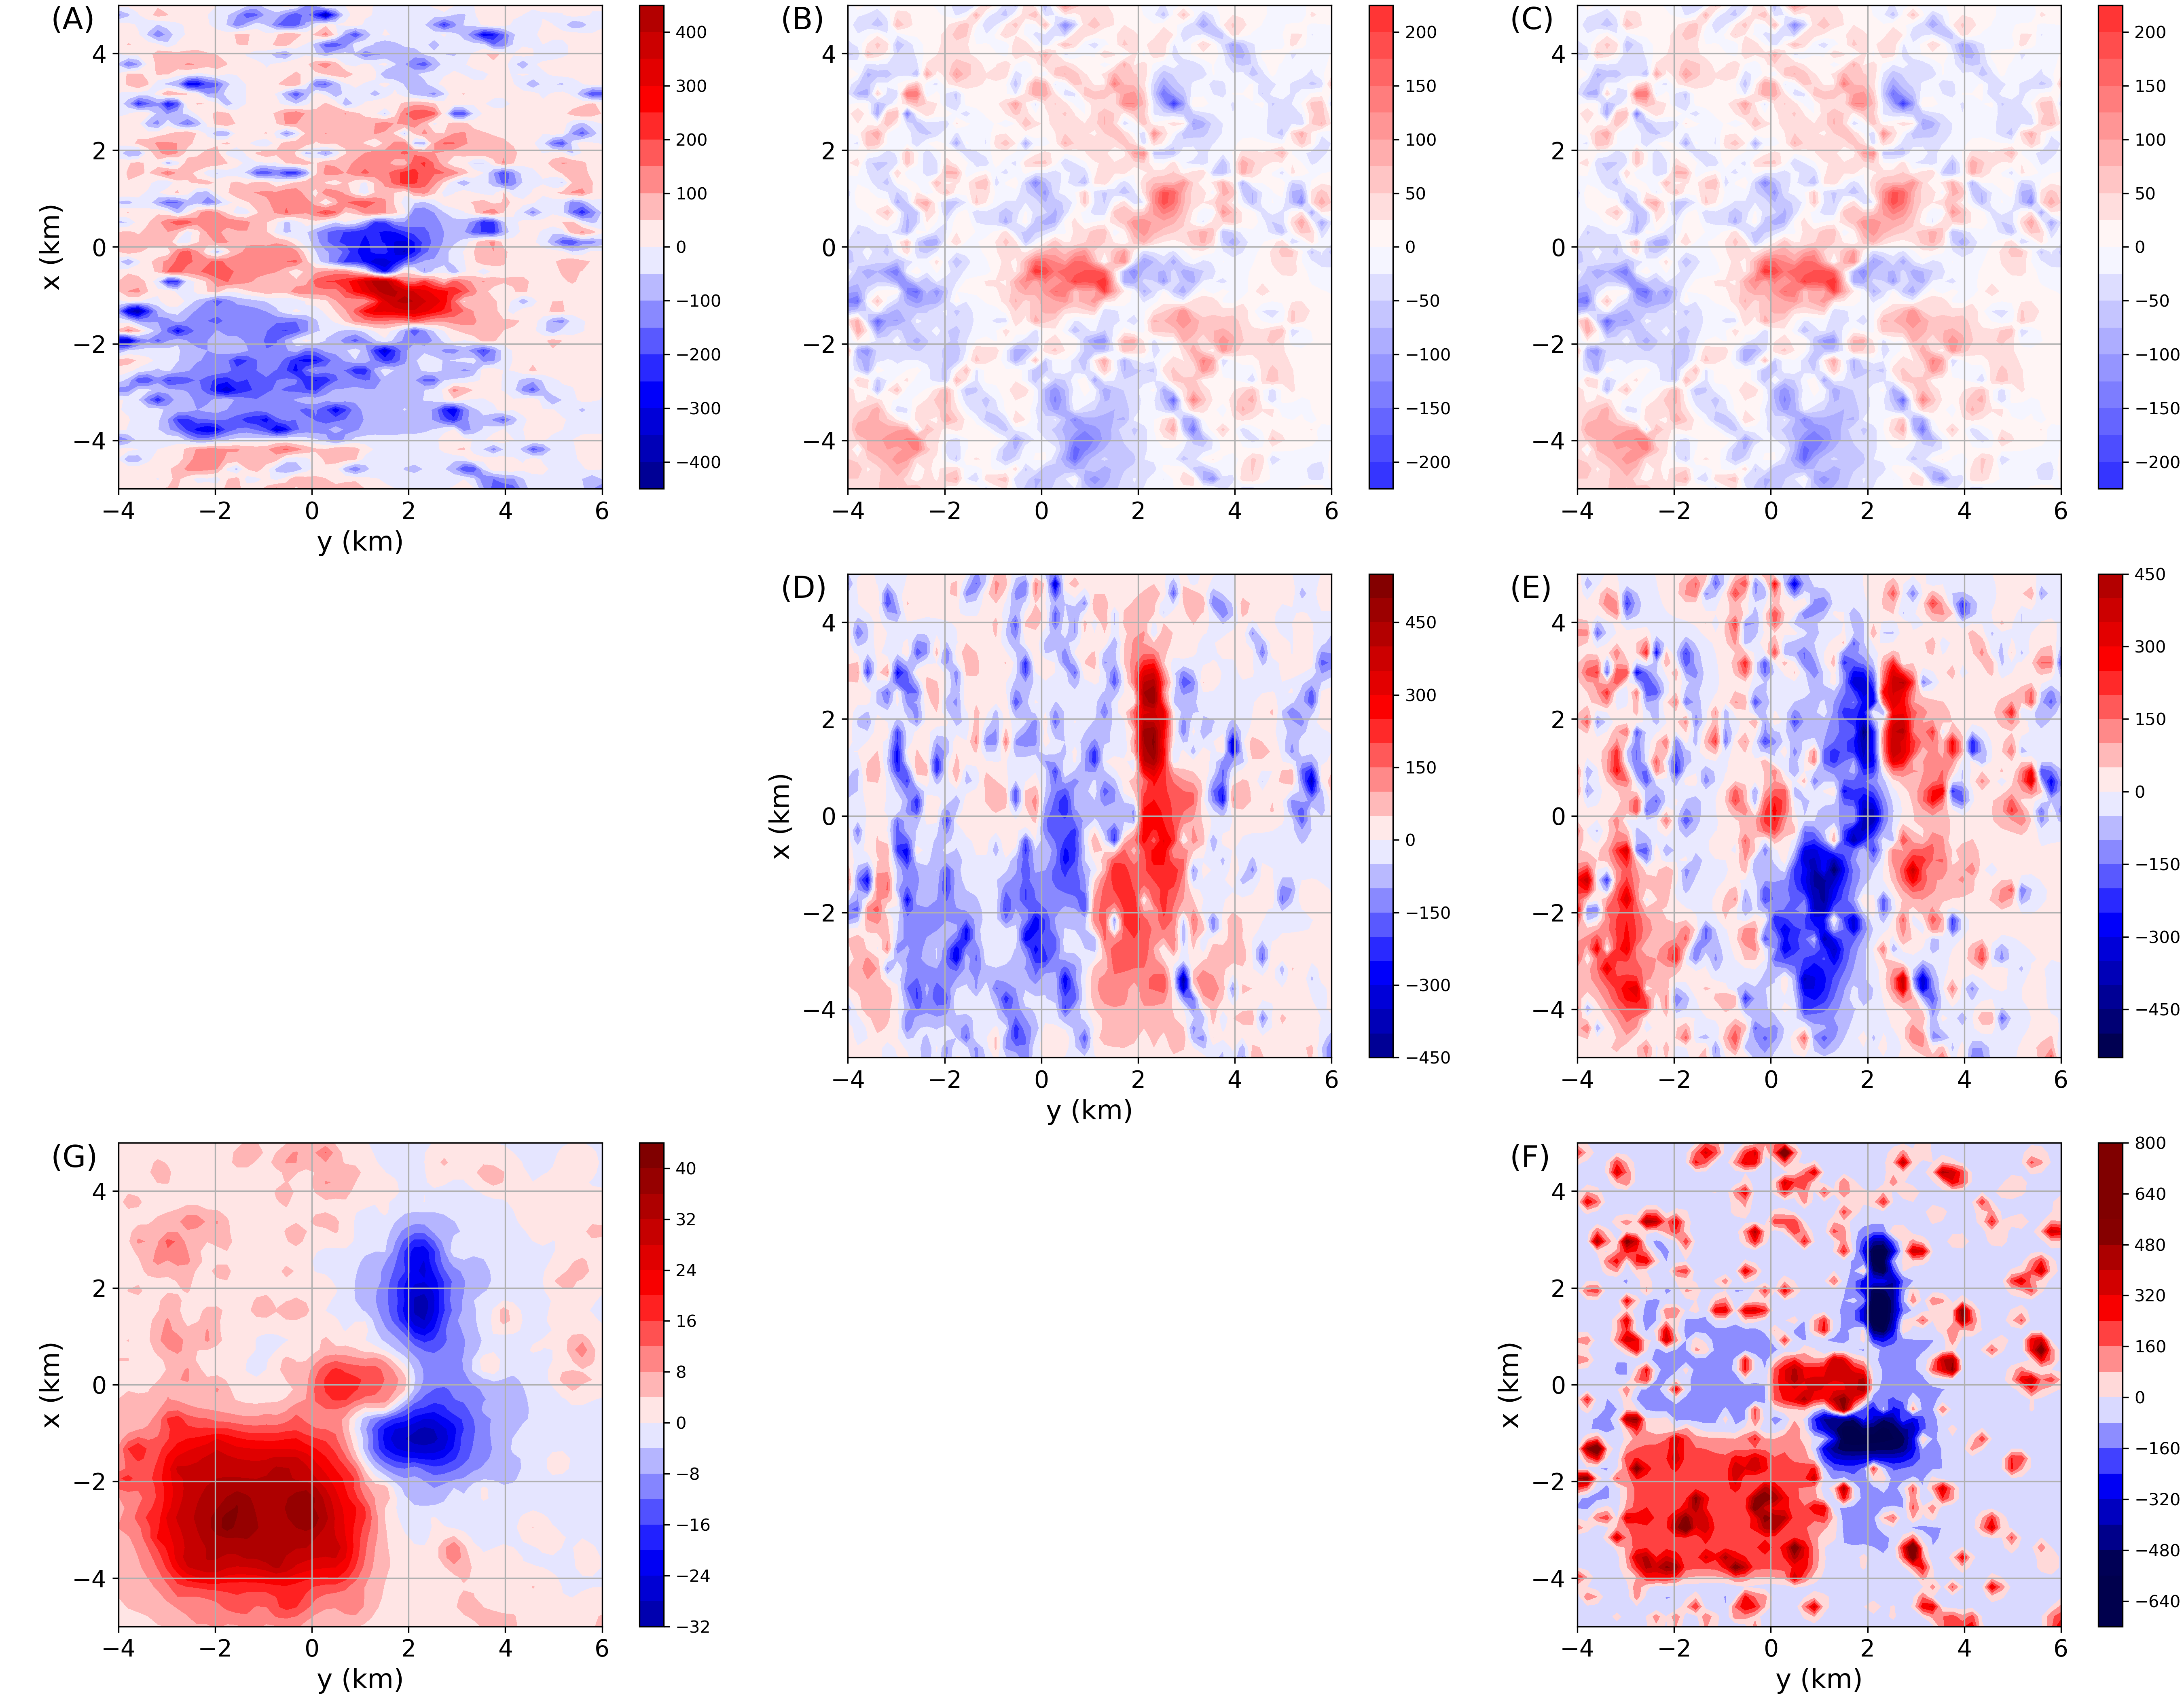
\includegraphics[width=9cm]{Fig/noise-free-data}
		\end{center}
	\caption{
		Noise-free gravity data produced by an ensemble of rectangular prisms (not shown). 
		The data are located on a regular grid of $50 \times 50$ points. 
		Panels \textbf{(A)}--\textbf{(F)} show, respectively, the $xx$, $xy$, $xz$, $yy$, $yz$ and
		$zz$ component of the gravity-gradient tensor in Eötvös (E).
		Panel \textbf{(G)} shows the gravity disturbance in milligals (mGal).
		}
	\label{fig:noise-free-data}
\end{figure}

\begin{figure}[htbp]
	\begin{center}
		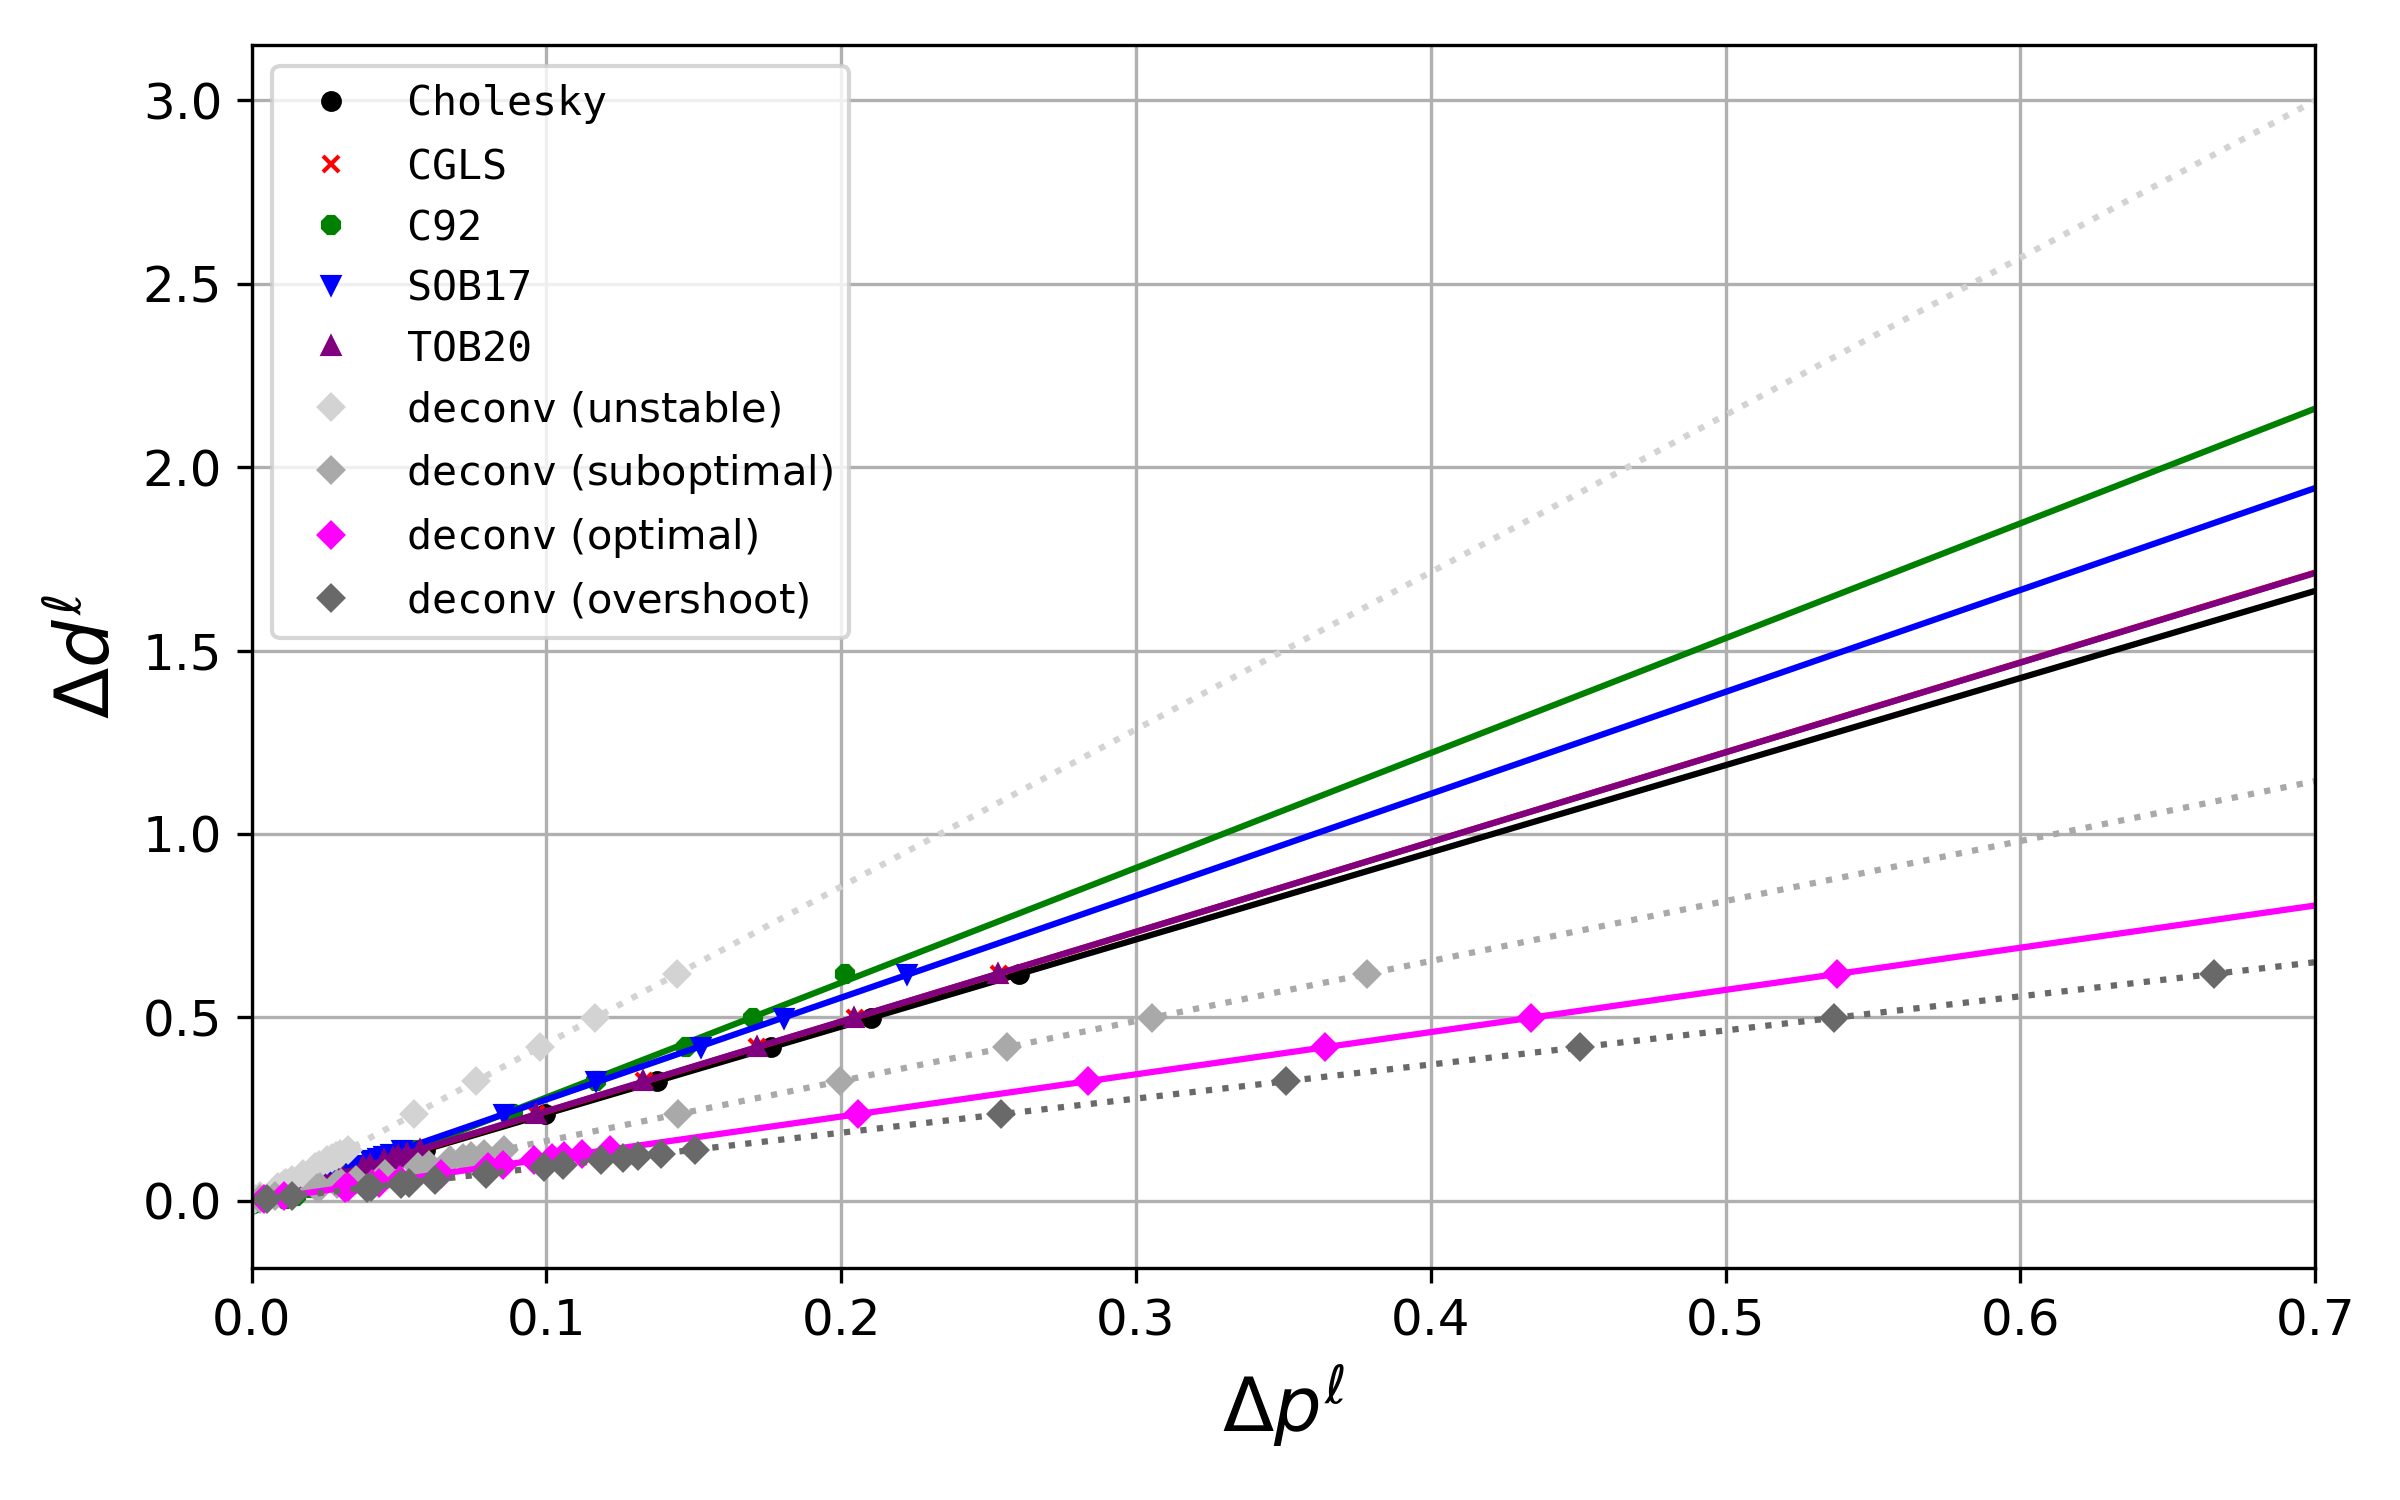
\includegraphics[width=9cm]{Fig/stability-comparison}
	\end{center}
	\caption{
		Numerical stability curves obtained for the $21$ synthetic gravity data sets 
		by using the Cholesky factorization with $\mu \approx 2 \times 10^{-2}$, 
		CGLS, iterative method (($\mathrm{SOB17}$)) and iterative deconvolution
		($\mathtt{TOB20}$) with $50$ iterations each (Algorithms \ref{alg:CGLS}, \ref{alg:SOB17} and \ref{alg:TOB20-22}) 
		and the direct deconvolution ($\mathtt{deconv.}$) computed with four different values for $\zeta$ 
		(equation \ref{eq:matrix-L-Wiener-deconvolution}): $0$, $10^{-18}$ (overshoot), $10^{-22}$ (optimal)
		and $10^{-28}$ (suboptimal).
		The stability parameter $\kappa$ (equation \ref{eq:condition-number}) obtained for the eight curves described above are $2.29$ ($\mathtt{Cholesky}$), $2.38$ 
		($\mathtt{CGLS}$), $3.25$ ($\mathtt{SOB17}$), $2.38$ ($\mathtt{TOB20}$), $4.83$, $1.59$, $1.11$ and $0.93$ ($\mathtt{deconv.}$ with null, suboptimal, optimal and overshoot $\zeta$).
		}
	\label{fig:stability-comparison}
\end{figure}

\begin{figure}[htbp]
	\begin{center}
		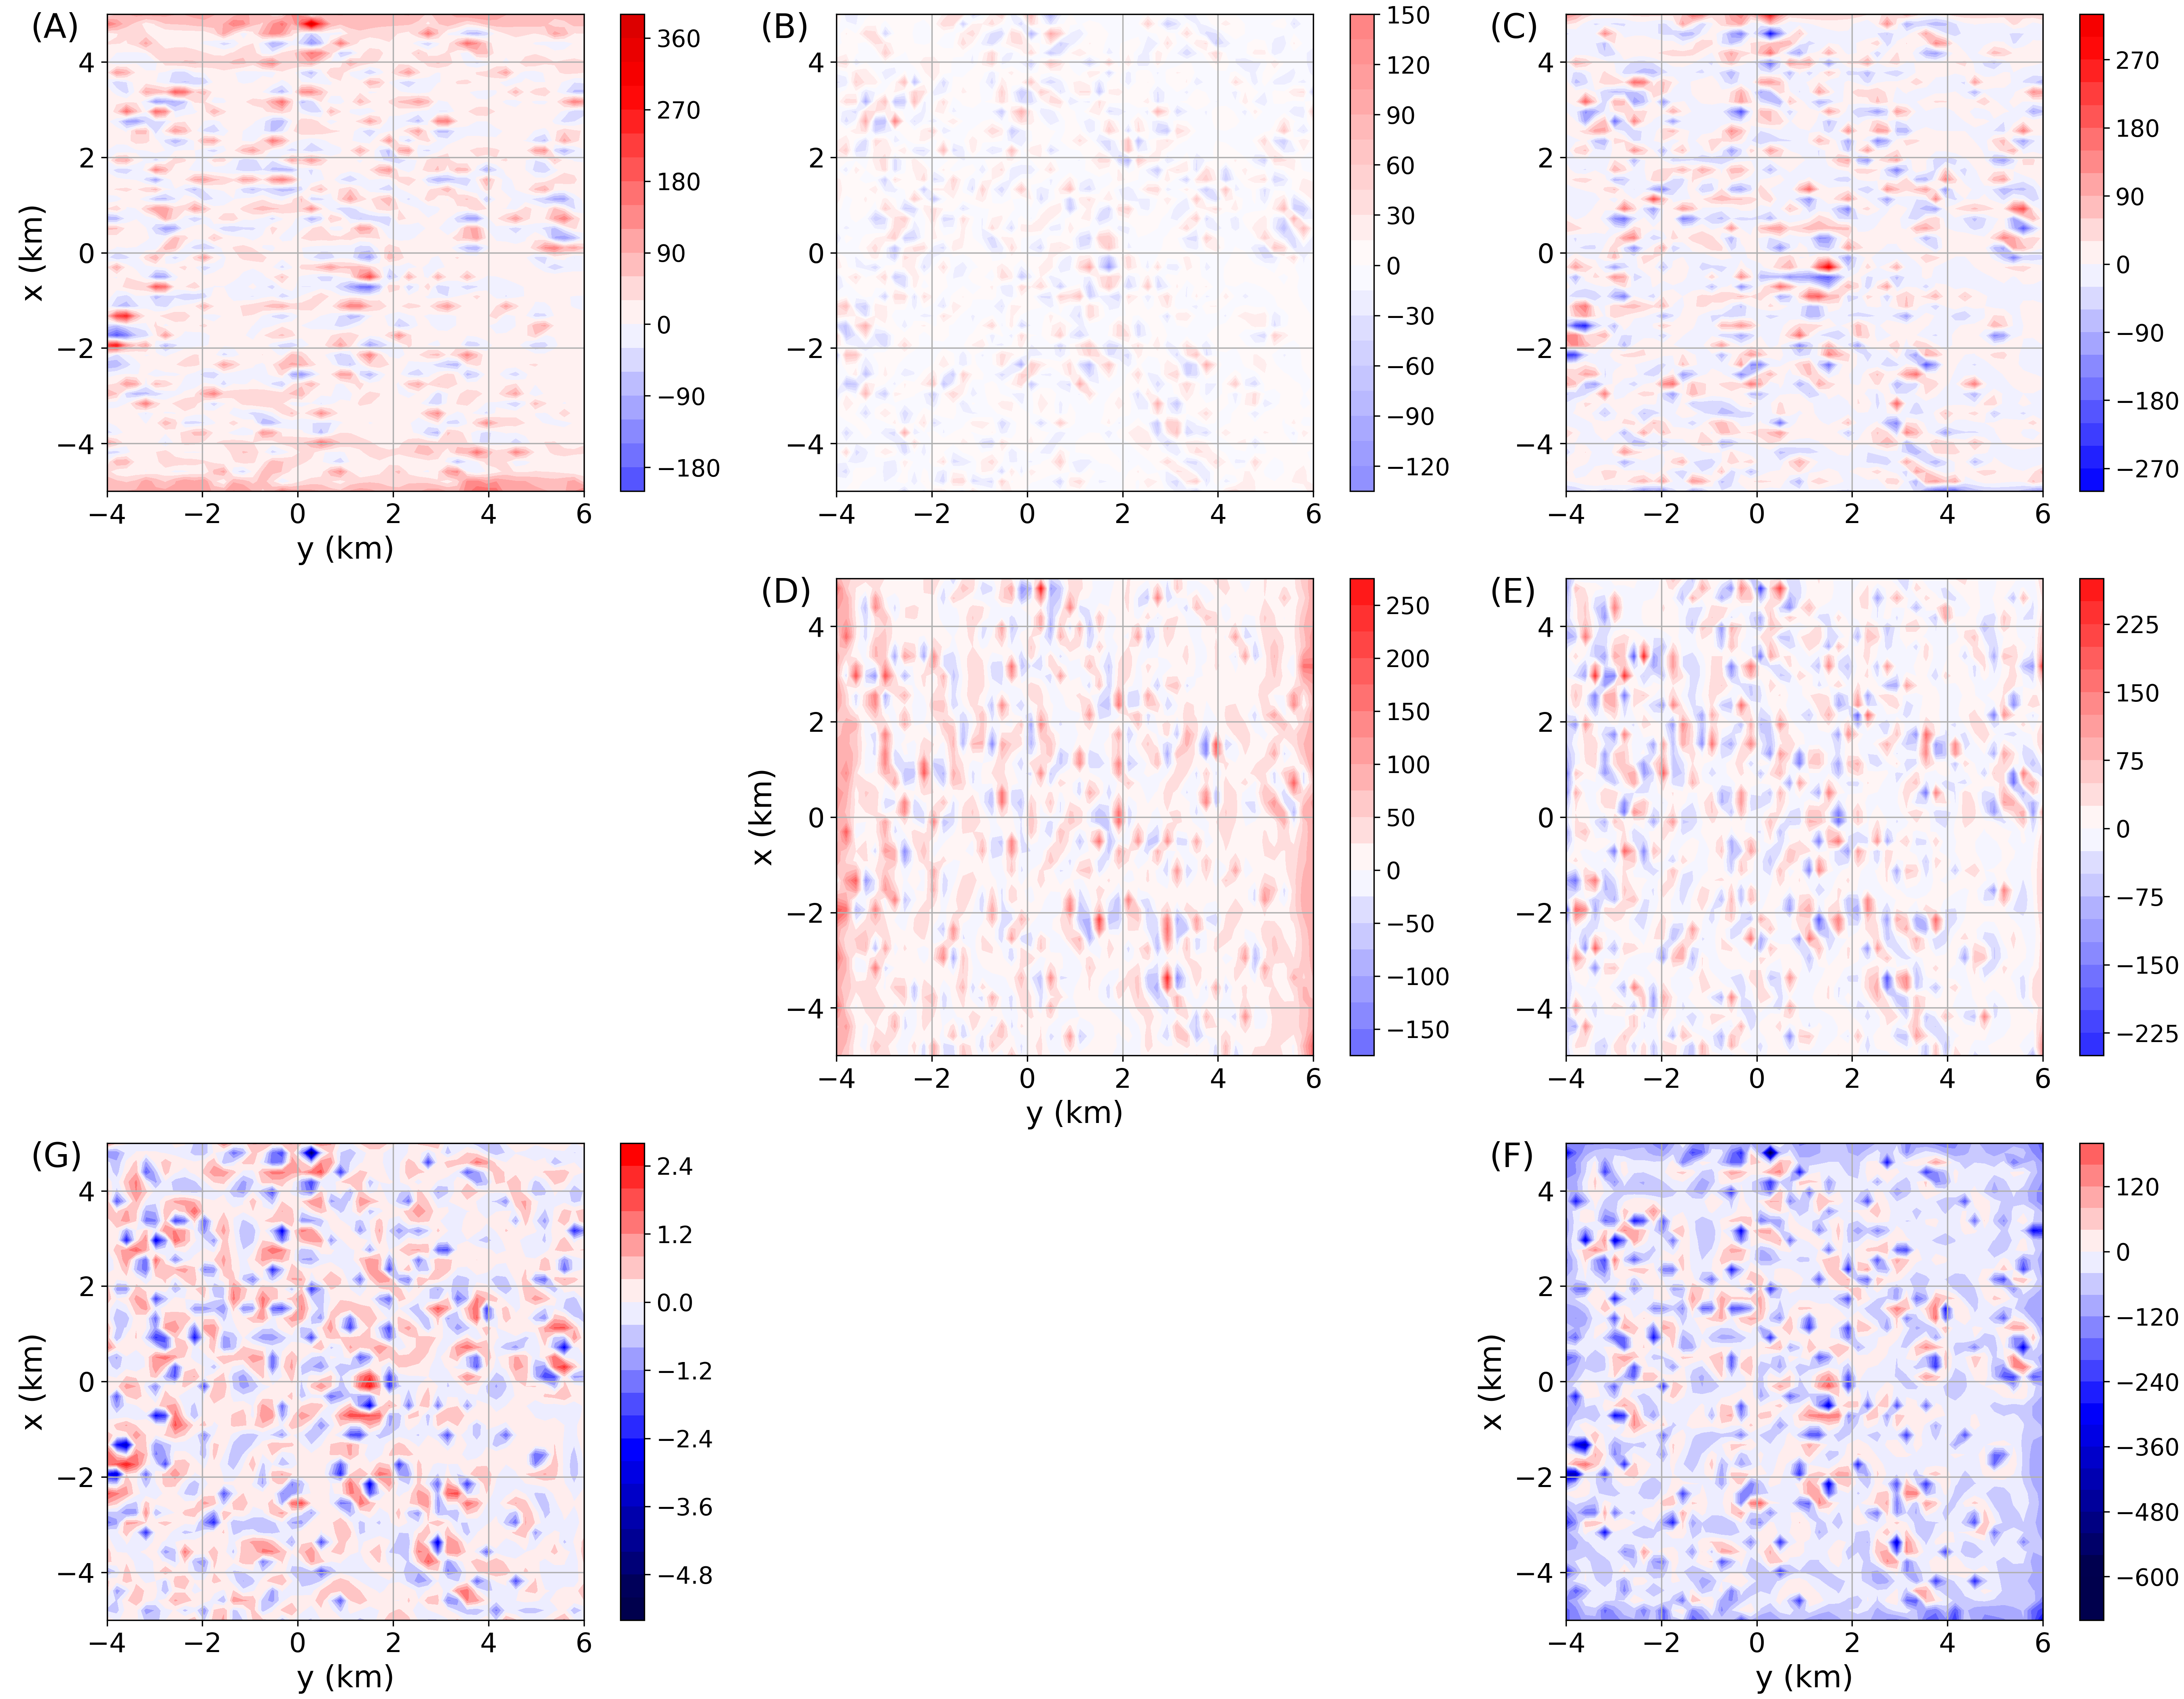
\includegraphics[width=10cm]{Fig/TOB20_residuals}
	\end{center}
	\caption{
		Residuals between the gravity data predicted by the equivalent layer estimated with the 
		iterative deconvolution ($\mathtt{TOB20}$) (Algorithm \ref{alg:TOB20-22}).
		The inverse problems was solved by using the noise-corrupted gravity 
		disturbance having the maximum noise level (not shown).
		Panels \textbf{(A)}--\textbf{(F)} show the residuals between the predicted and noise-free
		gravity gradient data (Figure \ref{fig:noise-free-data}) associated with the
		$xx$, $xy$, $xz$, $yy$, $yz$ and $zz$ components of the gravity-gradient tensor, respectively. 
		The values are in Eötvös.
		\textbf{(G)} Shows the residuals between the predicted and noise-corrupted gravity disturbances.
		The values are in milligals (mGal).
		}
	\label{fig:residuals-TOB20}
\end{figure}

\begin{figure}[htbp]
	\begin{center}
		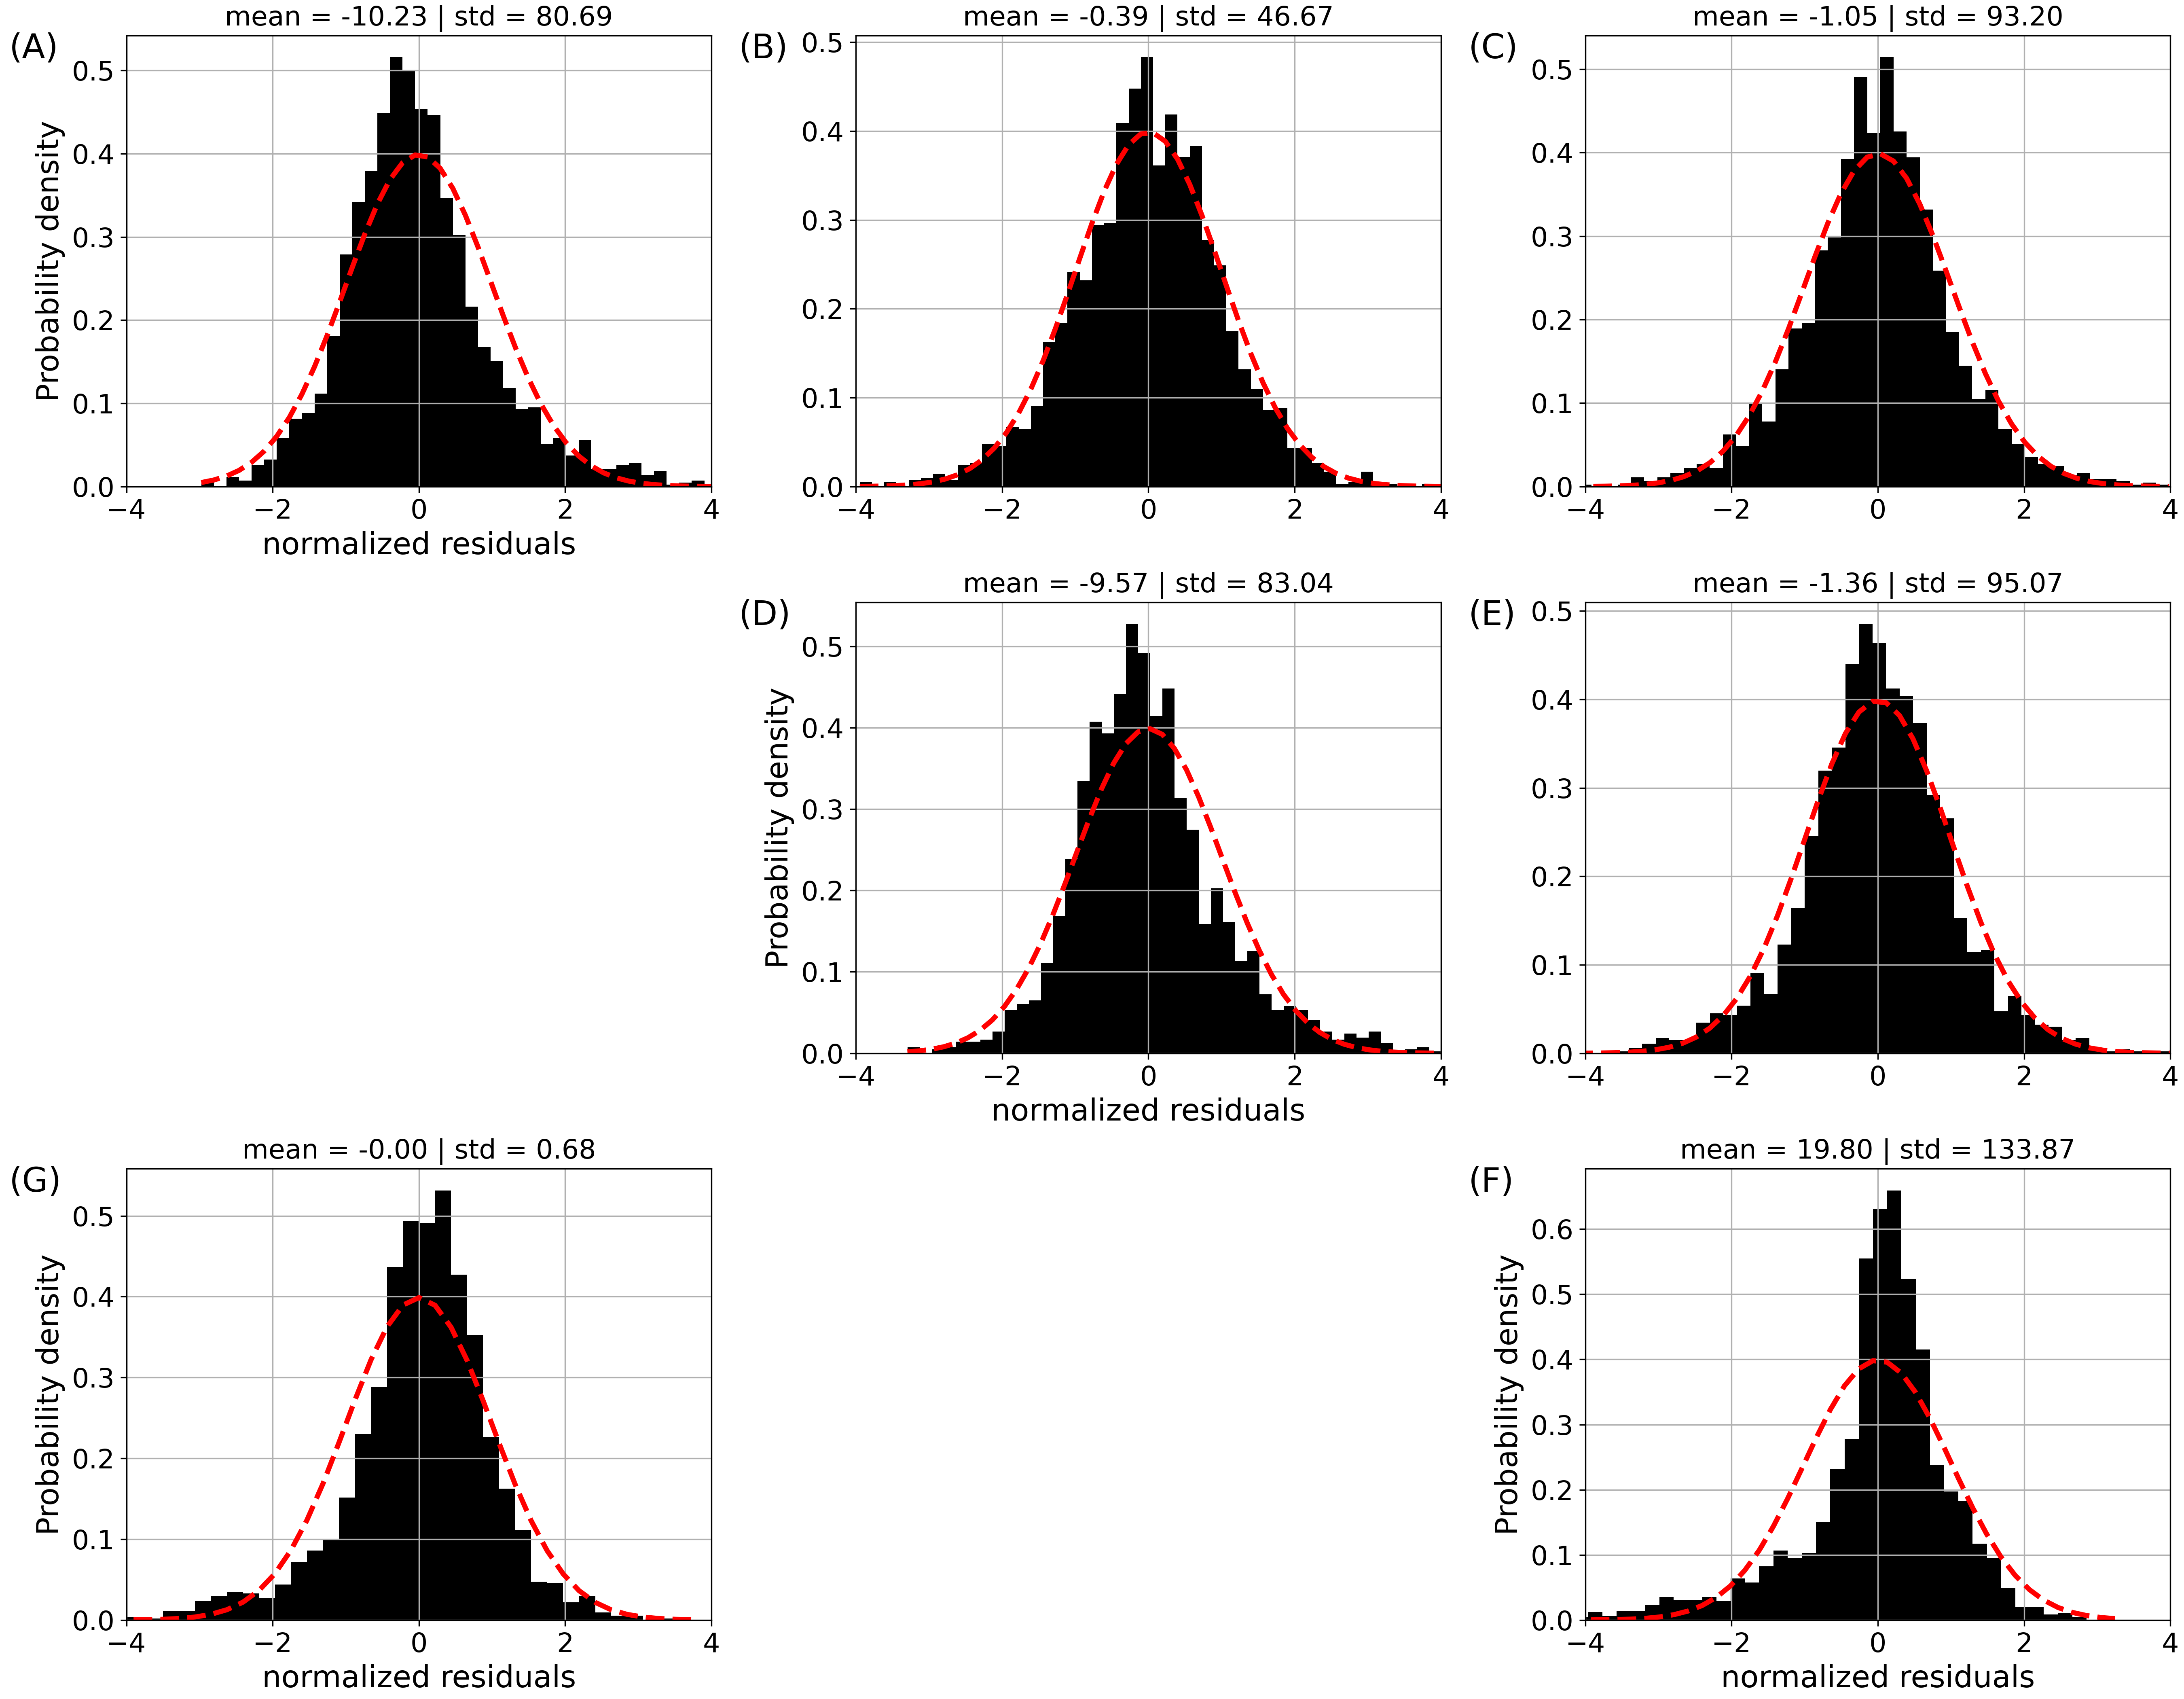
\includegraphics[width=10cm]{Fig/TOB20_histograms}
	\end{center}
	\caption{
		Histograms of the residuals shown in Figure \ref{fig:residuals-TOB20}.
		The residuals were normalized by removing the mean and dividing the difference
		by the standard deviation.
		Panels \textbf{(A)}--\textbf{(F)} show the histograms associated with the 
		$xx$, $xy$, $xz$, $yy$, $yz$ and $zz$ components of the gravity-gradient tensor, respectively. 
		\textbf{(G)} Shows the histogram of the residuals between the predicted and noise-corrupted gravity disturbances.
	}
	\label{fig:histograms-TOB20}
\end{figure}

\begin{figure}[htbp]
	\begin{center}
		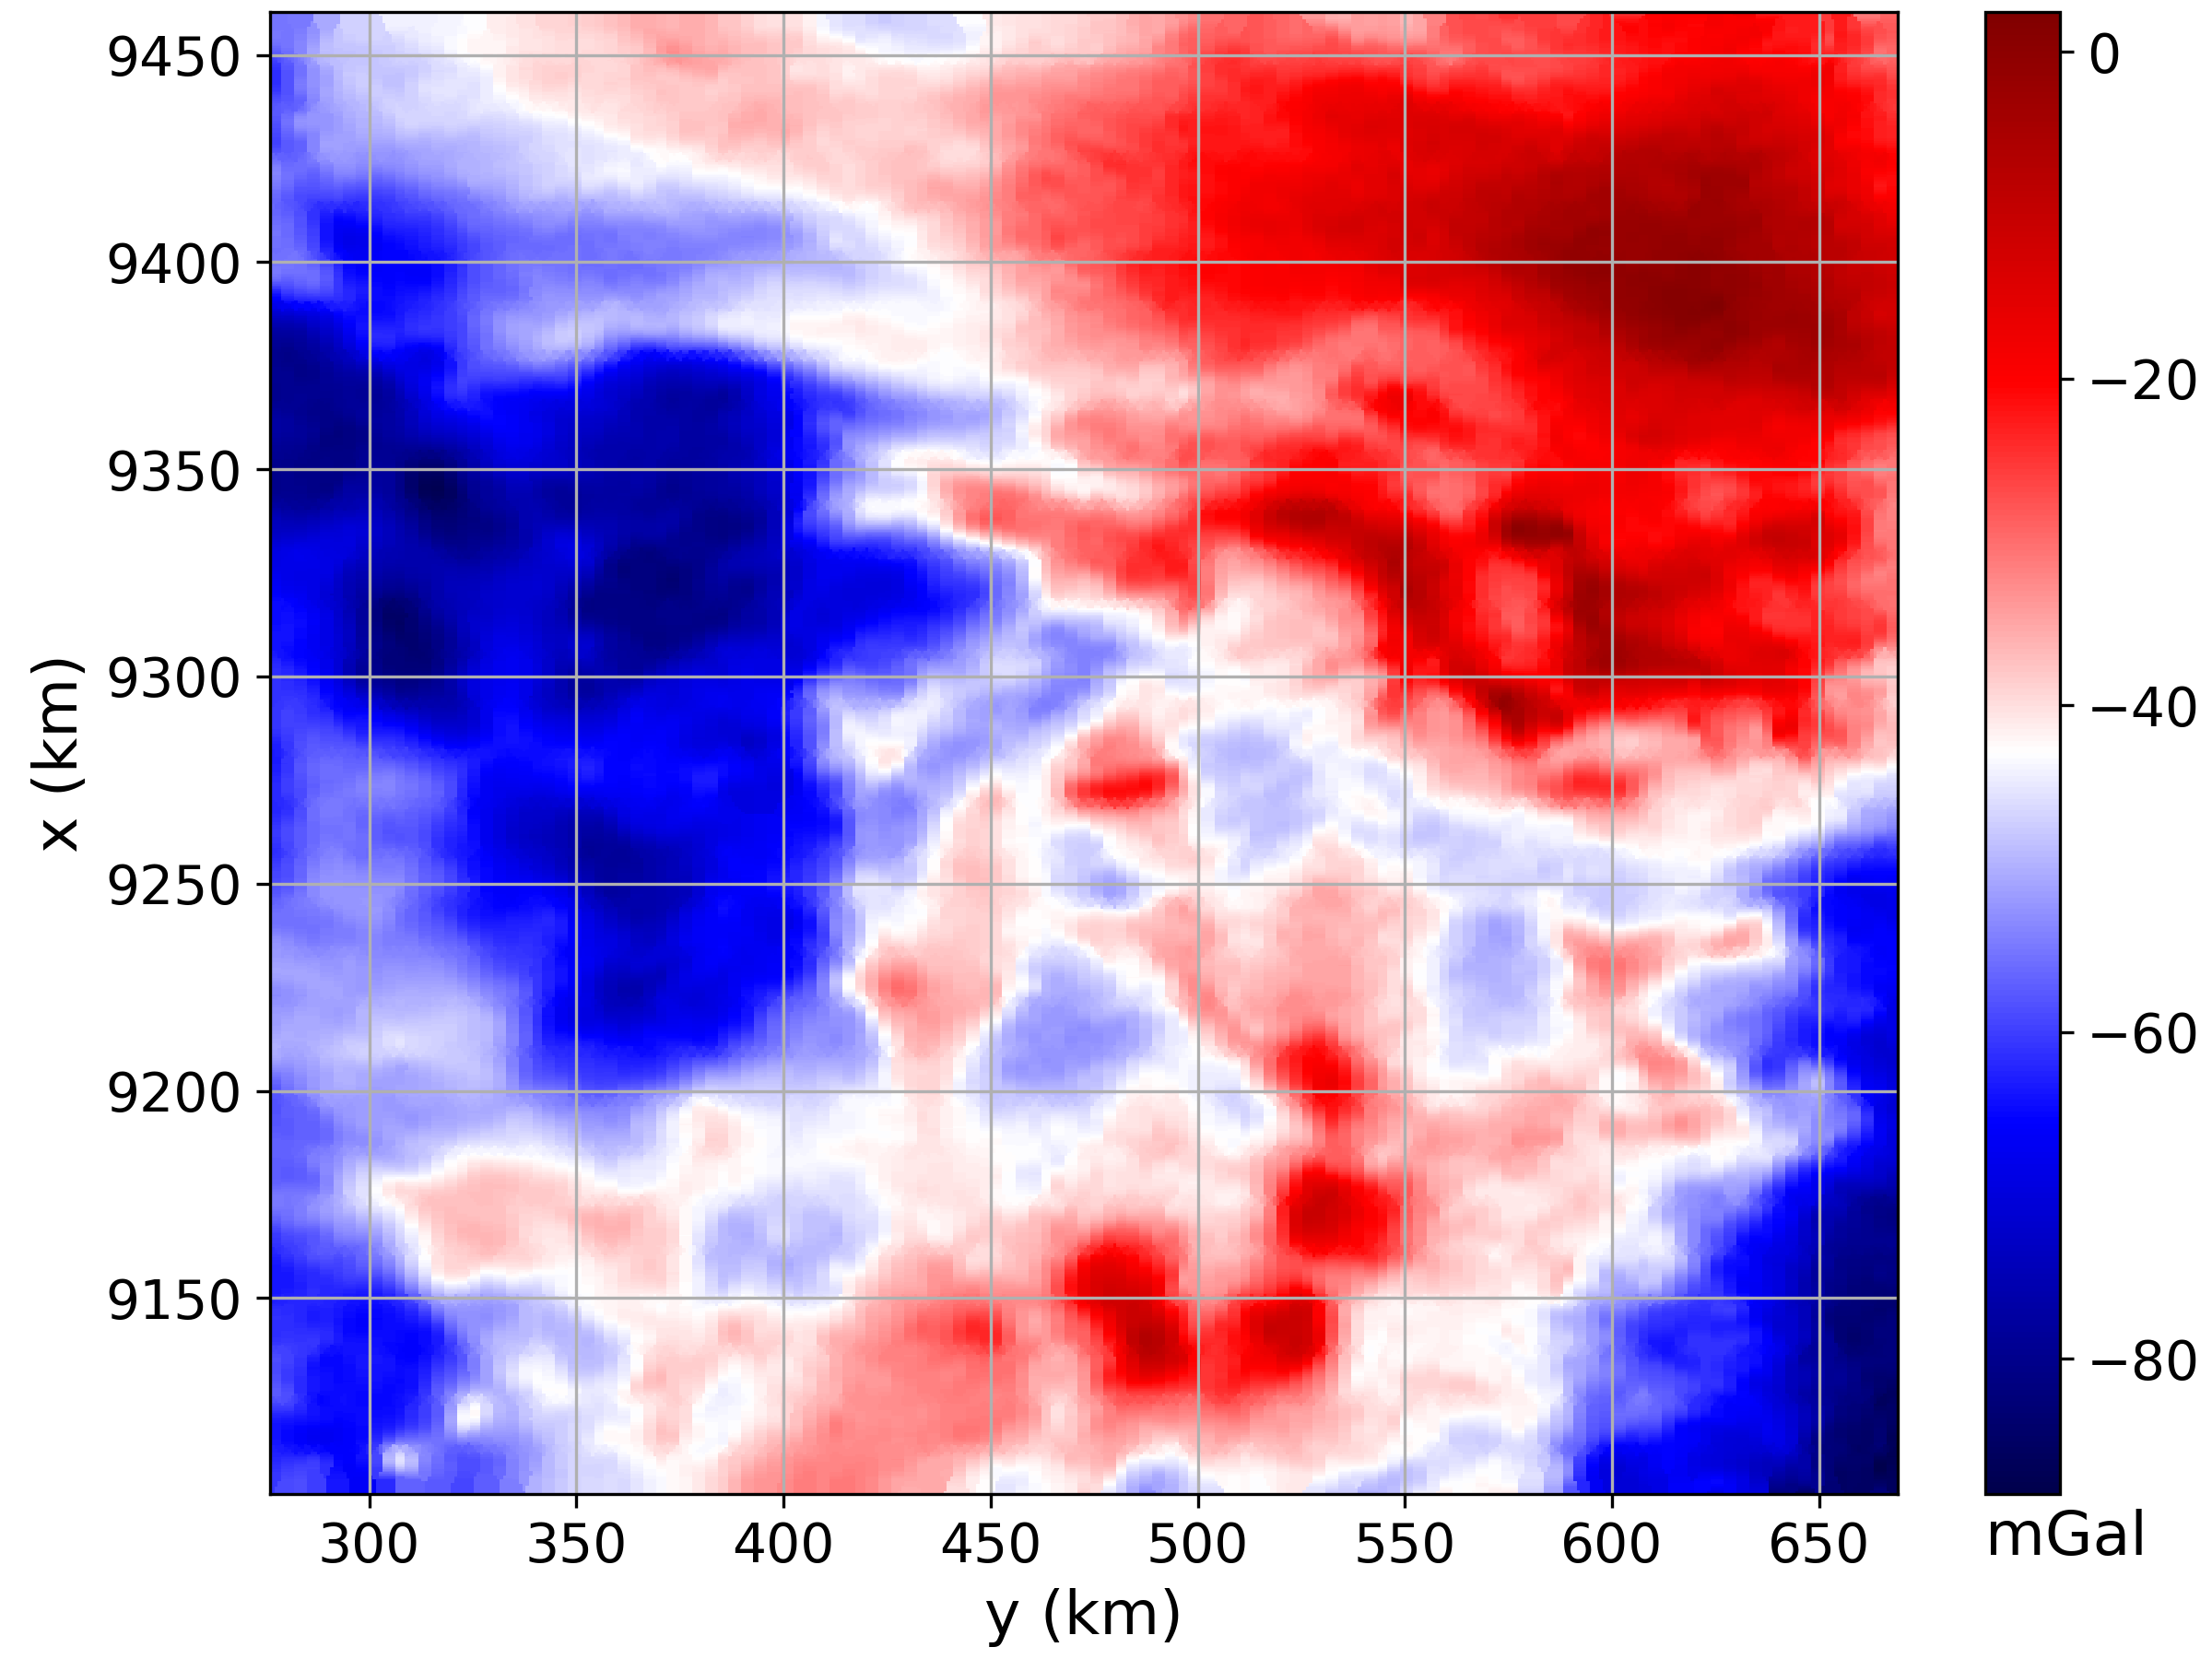
\includegraphics[width=10cm]{Fig/carajas_data}
	\end{center}
	\caption{
		Field aerogravimetric data over Caraj{\'a}s, Brazil. 
		There are $D = 500, 000$ observations located on regular grid of $1,000 \times 500$ poins.
		}
	\label{fig:carajas-data}
\end{figure}

\begin{figure}[htbp]
	\begin{center}
		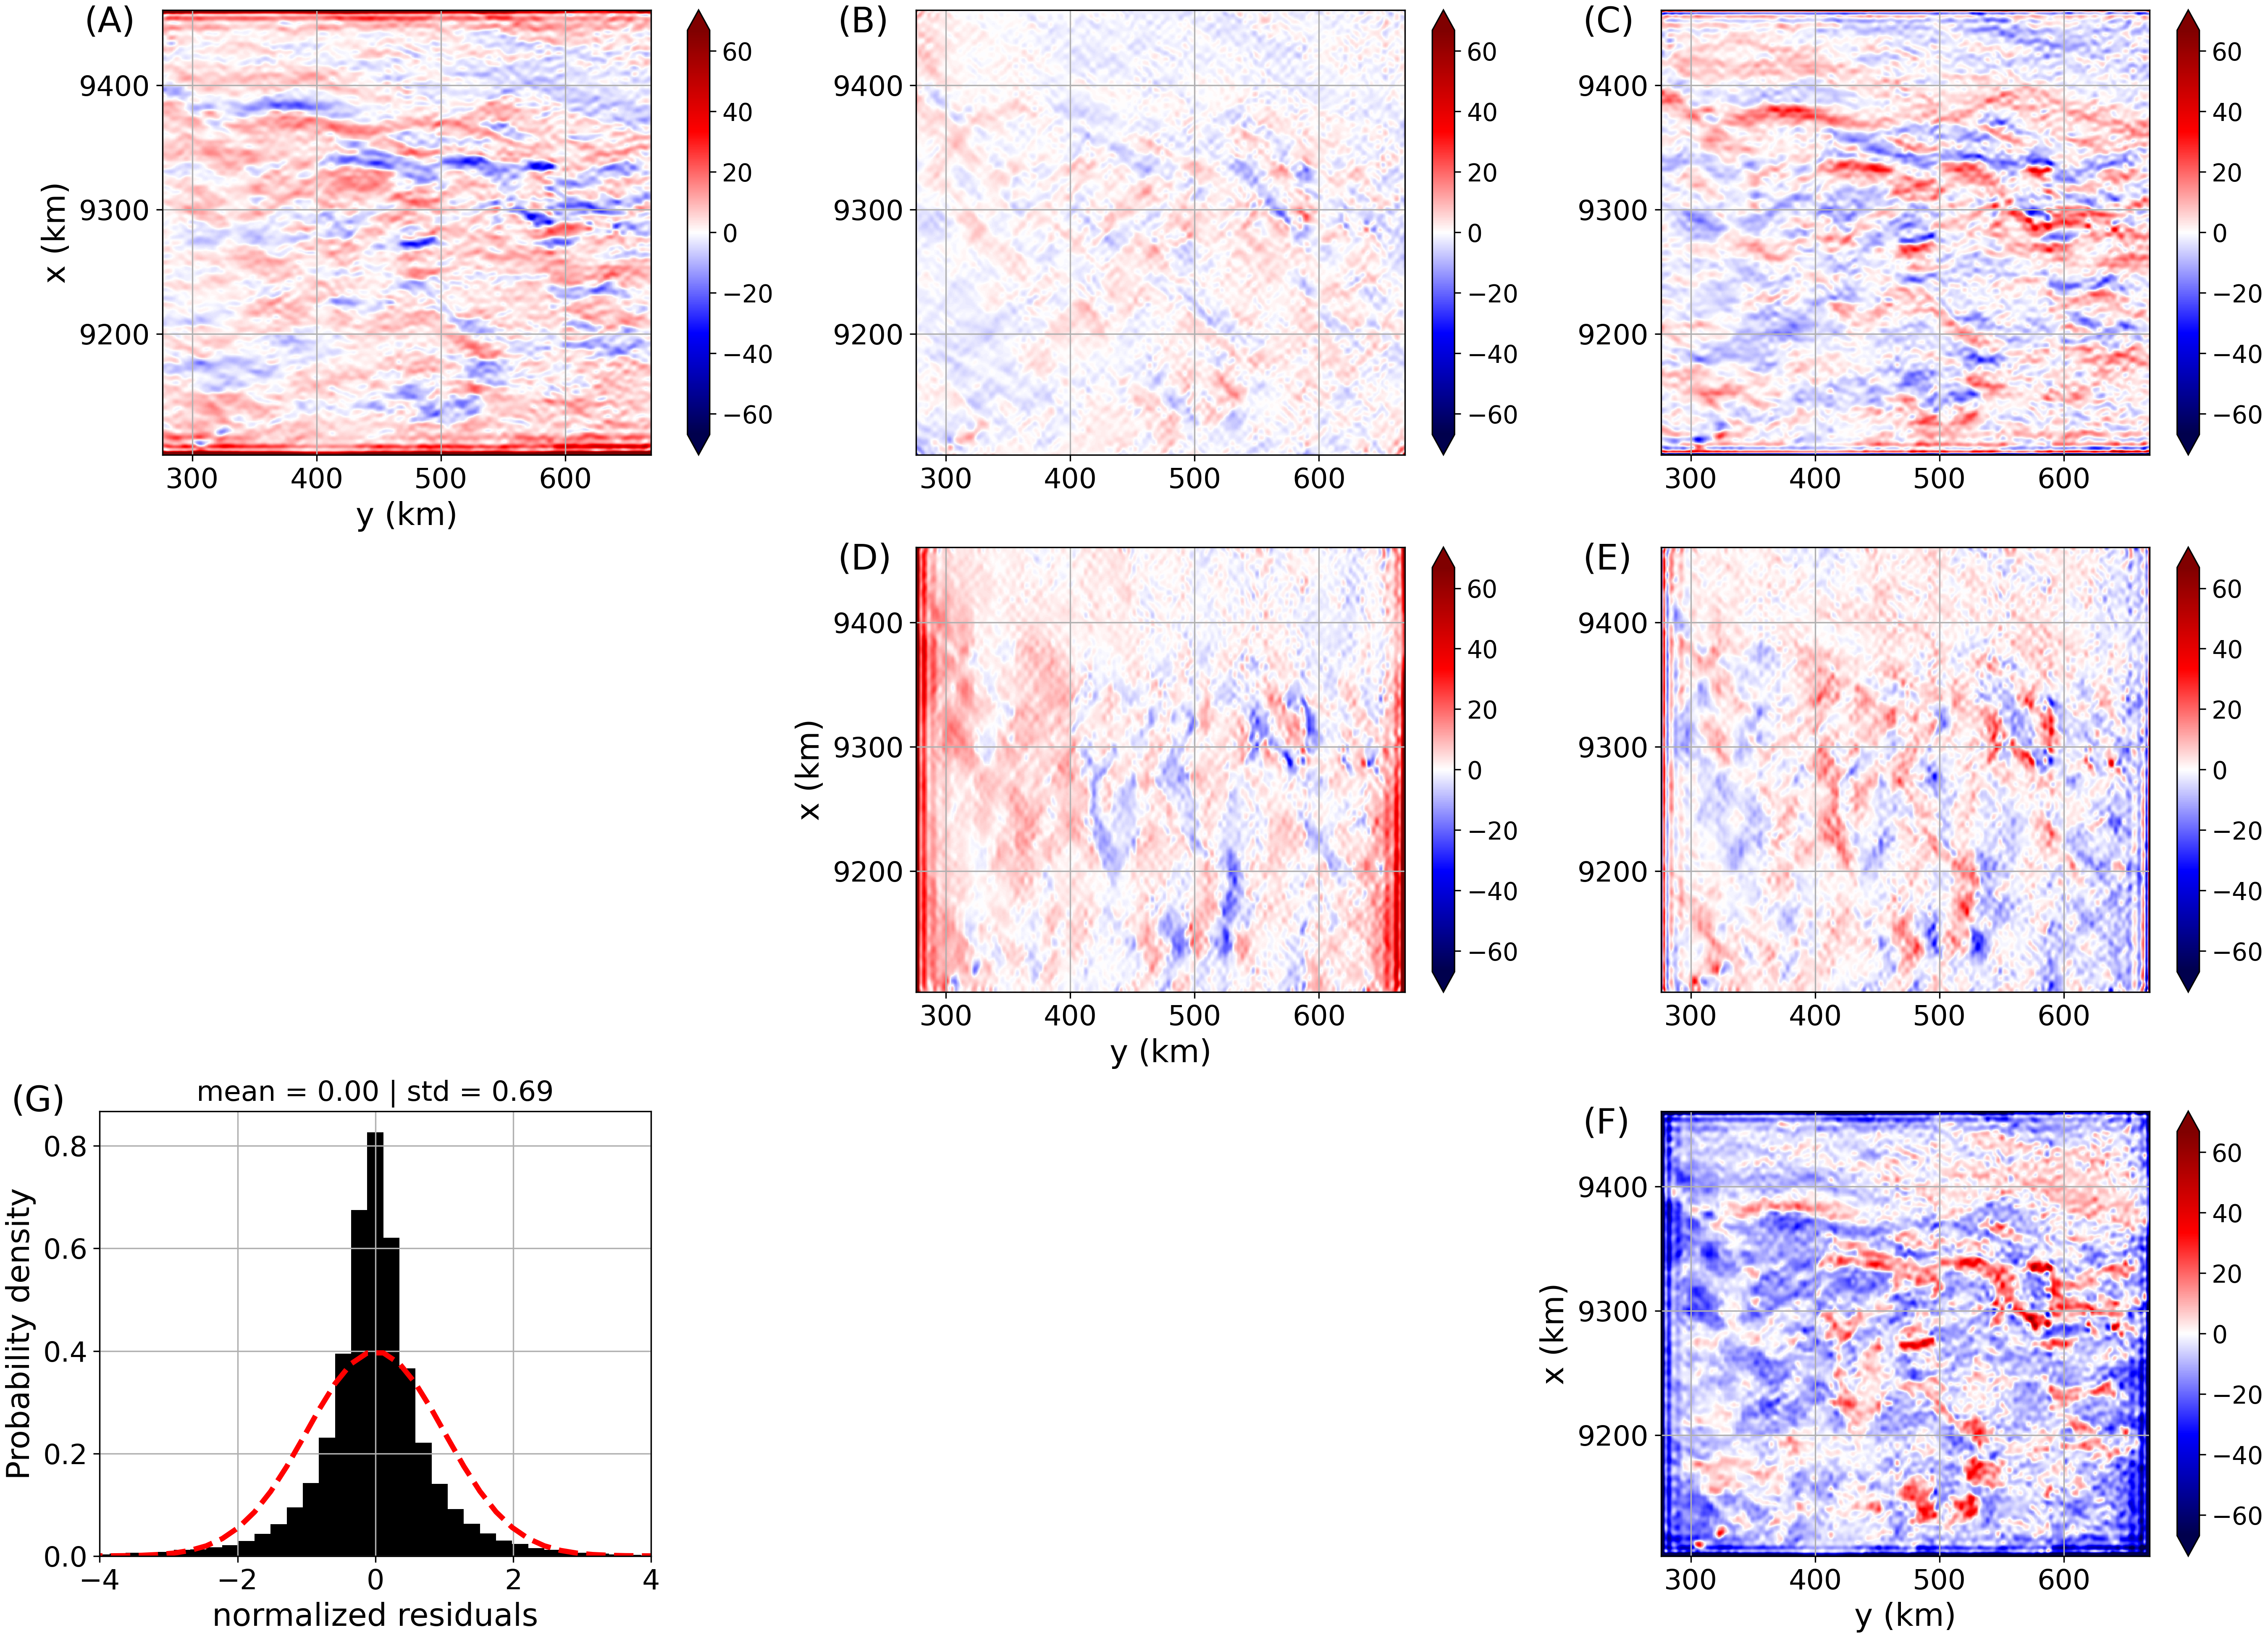
\includegraphics[width=10cm]{Fig/carajas_grav_gradient}
	\end{center}
	\caption{
		Estimated gravity-gradient tensor components over Caraj{\'a}s, Brazil.
		Panels \textbf{(A)}--\textbf{(F)} show, respectively, the $xx$, $xy$, $xz$, $yy$, $yz$ and
		$zz$ components of the gravity-gradient tensor in Eötvös.
		Panel \textbf{(G)} shows the histogram of the residuals between predicted data (not shown) and field data 
		(Figure \ref{fig:carajas-data}). 
		The residuals were normalized by removing the mean and dividing the difference
		by the standard deviation.
		The results were generated by applying the iterative deconvolution ($\mathtt{TOB20}$)
		(Algorithm \ref{alg:TOB20-22})
		with $50$ iterations.
		}
	\label{fig:carajas-grav-gradient}
\end{figure}

%%% If you are submitting a figure with subfigures please combine these into one image file with part labels integrated.
%%% If you don't add the figures in the LaTeX files, please upload them when submitting the article.
%%% Frontiers will add the figures at the end of the provisional pdf automatically
%%% The use of LaTeX coding to draw Diagrams/Figures/Structures should be avoided. They should be external callouts including graphics.


%\bibliographystyle{frontiersinSCNS_ENG_HUMS} %  for Science, Engineering and Humanities and Social Sciences articles, for Humanities and Social Sciences articles please include page numbers in the in-text citations
%\bibliographystyle{frontiersinHLTH&FPHY} % for Health and Physics articles
%\bibliography{test}

%\end{document}
